% Budget-constrained uplift targeting: a pre-registered study on the Hillstrom e-mail experiment.
% Layout follows the Bachelor's Project Thesis format: A4, two columns, author-year (APA) citations.
% Compile with pdfLaTeX + BibTeX (Overleaf default). Figures in figures/, references in references.bib.
\documentclass[10pt,twocolumn]{article}

\usepackage[a4paper,top=2.2cm,bottom=2.4cm,left=1.9cm,right=1.9cm,columnsep=0.7cm]{geometry}
\usepackage[T1]{fontenc}
\usepackage[utf8]{inputenc}
\usepackage{amsmath}
\usepackage{newtxtext,newtxmath}
\usepackage{graphicx}
\usepackage{booktabs}
\usepackage{caption}
\usepackage{xcolor}
\usepackage[natbibapa]{apacite}
\usepackage[hidelinks]{hyperref}
\usepackage{microtype}

\setcounter{secnumdepth}{3}
\captionsetup{font=small,labelfont=bf}
\setlength{\abovecaptionskip}{4pt}
\setlength{\textfloatsep}{10pt}

% ---- edit before publishing ---------------------------------------------------------------
\newcommand{\reporttype}{Research Project Report}
\newcommand{\authorline}{Simion Polivencu, \textit{student number}, \textit{e-mail}}
\newcommand{\supervisorline}{\textit{Supervisor (if any)}}
\newcommand{\repourl}{\url{https://github.com/USERNAME/budgeted-uplift}}
% --------------------------------------------------------------------------------------------

\newcommand{\E}{\mathbb{E}}
\newcommand{\Prob}{\mathbb{P}}
\newcommand{\ind}{\mathbf{1}}
\newcommand{\tauh}{\hat{\tau}}
\newcommand{\muh}{\hat{\mu}}
\newcommand{\CI}[2]{\ensuremath{[#1,\,#2]}}
\DeclareMathOperator*{\argmax}{arg\,max}

\begin{document}

\twocolumn[
\begin{@twocolumnfalse}
\begin{center}
{\LARGE\bfseries When Does Uplift Targeting Pay Off?\\[2pt]
A Pre-registered, Budget-Constrained Study of the\\[2pt] Hillstrom E-mail Experiment\par}
\vspace{0.6em}
{\large\itshape \reporttype\par}
\vspace{0.4em}
{\authorline\par}
{\supervisorline\par}
\end{center}
\vspace{0.6em}
\noindent\textbf{Abstract:} Uplift models promise to send a promotion only to the customers it
persuades, but their value is rarely tested end to end: from a randomised experiment, through
heterogeneous-effect estimation and budget-constrained optimisation, to an unbiased estimate of the
money the resulting policy earns. This project runs that full pipeline on the Hillstrom e-mail
experiment (64{,}000 customers, three randomised arms) under a release protocol in which every
analysis choice is frozen in a commit before it is run. Five uplift learners fail to rank customers
better than random on two-week spend, and the model-targeted policy does not beat the one-line rule
``send the better e-mail to a random subset'' at any budget. A semi-synthetic positive control on
the same covariates and assignment shows that the same code recovers a known effect (correlation of
estimated and true effects up to $0.83$; $+\$0.50$ $\CI{0.27}{0.75}$ per customer over random
targeting at a 30\% budget). A sweep over effect heterogeneity and sample size explains the null: at
Hillstrom's size a single experiment detects a real gain over the best single arm in only 5 to 25\%
of replications unless most of the effect is concentrated in a third of customers. Further,
repeated cross-fitting narrows policy-value intervals by 37 to 58\%; a profit objective recovers the
known profit-optimal budget; doubly robust policy trees never outperform estimate-then-optimise;
plug-in chance constraints on random voucher uptake are defeated by the optimiser's curse, which a
recalibration cannot repair while a conservative bootstrap bound can; and a budgeted
Thompson-sampling bandit beats or ties every experiment-then-target design.
\vspace{1.4em}
\end{@twocolumnfalse}
]

% =========================================================================================
\section{Introduction}
\label{sec:intro}

Marketing budgets are finite, so a firm that can send two different promotional e-mails must
decide \emph{who} receives \emph{which} e-mail, and how much to spend in total. Uplift modelling
\citep{radcliffe2007,gutierrez2017} answers the first question by estimating, for each customer, the
conditional average treatment effect (CATE) of each promotion and targeting those with the largest
predicted lift. Whether such estimates are \emph{good enough to change a decision} is a different
question, and it is the one a business cares about.

Answering it requires connecting four steps that are usually studied separately: a randomised
experiment that identifies causal effects; a model of how those effects vary across customers; an
optimisation that turns noisy estimates into a feasible allocation under a budget; and an unbiased,
uncertainty-quantified evaluation of the resulting policy. Errors compound along this chain: a
learner that is ``better than random'' on a ranking metric may still lose money once the budget is
spent, and an optimiser fed noisy estimates systematically over-promises \citep{smith2006}.

\paragraph{Background.}
Uplift modelling originated in direct marketing, where \citet{radcliffe2007} introduced the Qini
curve; \citet{gutierrez2017} connect it to the potential-outcomes framework
\citep{rubin1974,imbens2015}. Multi-treatment uplift is treated by \citet{zhao2017} and benchmarked
by \citet{olaya2020}. Meta-learners reduce CATE estimation to supervised learning
\citep{kunzel2019,kennedy2023,nie2021}, causal forests adapt random forests to effect estimation
\citep{wager2018,athey2019grf}, and double/debiased machine learning \citep{chernozhukov2018} provides
the cross-fitting framework used for evaluation. Inverse-propensity weighting \citep{horvitz1952}
and doubly robust estimators \citep{robins1994,dudik2011} evaluate a policy from randomised data, and
policy learning maximises such estimates directly \citep{kitagawa2018,athey2021}. Assigning one of
several costly treatments under a budget is a multiple-choice knapsack \citep{sinha1979,kellerer2004}
with fast Lagrangian solutions \citep{everett1963}; chance-constrained programming
\citep{charnes1959} handles random costs; Thompson sampling \citep{thompson1933,russo2018,eckles2014}
and bandits with knapsacks \citep{badanidiyuru2018} address sequential budgeted decisions.

\paragraph{Approach.}
This project runs the full chain on the Hillstrom e-mail experiment \citep{hillstrom2008}, with an
emphasis on credibility rather than on a new estimator. Every release freezes its configuration in a
version-control commit \emph{before} the code that uses it is run, in the spirit of
\citet{nosek2018}; real covariates and assignment are combined with simulated outcomes of known CATE
as a positive control; and negative results are reported rather than tuned away.

\paragraph{Research question.}
\emph{Can heterogeneous treatment effects estimated from a randomised experiment pick who gets which
e-mail better than simple rules, at every budget, and if not, why not?} Section~\ref{sec:problem}
formalises the problem, Section~\ref{sec:theory} presents the estimators and solvers,
Section~\ref{sec:method} the data and experimental design, Section~\ref{sec:results} the results and
Section~\ref{sec:conclusions} the conclusions.

% =========================================================================================
\section{Problem Formulation}
\label{sec:problem}

\subsection{Causal Setting}
Customer $i$ has covariates $X_i$, receives arm $T_i\in\{0,1,2\}$ (no e-mail, Mens, Womens) and has
potential outcomes $Y_i(a)$. Under SUTVA and randomisation with known propensity
$e(a)=\Prob(T=a)=1/3$, the conditional effect of arm $a$,
\begin{equation}
  \tau_a(x) = \E\big[Y(a)-Y(0)\mid X=x\big],
\end{equation}
is identified. The propensity is plugged in rather than estimated everywhere except in a
deliberately confounded robustness check.

\subsection{Budgeted Allocation}
With $x_{ia}\in\{0,1\}$ indicating that customer $i$ receives arm $a\in\{1,2\}$, costs $c_a$ and
budget $B$, the allocation problem is the multiple-choice knapsack \citep{sinha1979}
\begin{equation}
\begin{aligned}
  \max_{x}\ \ & \textstyle\sum_{i}\sum_{a} \tauh_{ia}\, x_{ia}\\
  \text{s.t.}\ \ & \textstyle\sum_{a} x_{ia}\le 1\ \ \forall i, \qquad \sum_{i}\sum_{a} c_a\, x_{ia}\le B.
\end{aligned}
\label{eq:ip}
\end{equation}
Hillstrom contains no cost data; we assume \$0.10 per Mens and \$0.08 per Womens e-mail and express a
budget as a fraction $f$ of the cost of e-mailing everyone at the average cost, $B=f\cdot n\cdot\bar c$
with $\bar c=\$0.09$.

\subsection{Profit Objective}
With gross margin $m$ (assumed 30\%; sensitivity 15\% and 50\%) and policy value $V(\pi)$, the
incremental profit of a policy that assigns arm probabilities $\pi(a\mid x)$ is
\begin{equation}
  \Pi(\pi) = m\,\big[V(\pi)-V(\pi_0)\big] - \textstyle\frac1n\sum_i\sum_a \pi(a\mid X_i)\,c_a,
\end{equation}
where $\pi_0$ sends nothing. The \emph{profit-targeted} policy replaces $\tauh_{ia}$ by
$m\tauh_{ia}-c_a$ in \eqref{eq:ip}, so it e-mails only customers whose expected margin exceeds the
e-mail cost and may leave budget unspent.

\subsection{Random Uptake and Chance Constraints}
Suppose each e-mail carries a \$5 voucher, paid on every purchase by a targeted customer. With
purchase probability $p_{ia}$, e-mailing $i$ with arm $a$ costs $c_a+5p_{ia}$ in expectation with
variance $25\,p_{ia}(1-p_{ia})$, so the campaign cost $C(\pi)$ is random. A mean-budget policy only
requires $\E[C]\le B$; a chance-constrained policy \citep{charnes1959} requires
\begin{equation}
  \Prob\big(C(\pi)>B\big)\le\varepsilon \;\Longleftarrow\;
  \E[C(\pi)] + z_{1-\varepsilon}\sqrt{\operatorname{Var}[C(\pi)]}\le B,
\end{equation}
with $\varepsilon=0.05$.

\subsection{Sequential Allocation}
In the sequential variant, a campaign of 64{,}000 customers arrives in 16 batches of 4{,}000; the
outcomes of a batch are observed before the next is allocated, and one total budget ($f=0.3$) is
paced evenly. The question becomes whether a policy should keep learning while it spends.

% =========================================================================================
\section{Theoretical Framework}
\label{sec:theory}

\subsection{Average Effects}
For arm $a$ against control we use the difference in means with a Welch interval and the fully
interacted regression adjustment of \citet{lin2013},
\begin{equation}
  Y_i = \alpha + \beta D_i + (X_i-\bar X)^{\top}\gamma + D_i (X_i-\bar X)^{\top}\delta + \varepsilon_i,
\end{equation}
where $D_i=\ind[T_i=a]$ and $\hat\beta$ estimates the ATE with HC2 standard errors; with past spend
as the only covariate this is CUPED \citep{deng2013}.

\subsection{CATE Learners}
All base models are LightGBM regressors \citep{ke2017}.

\subsubsection{S- and T-learner}
The S-learner fits $\mu(x,a)$ on $[x,\text{onehot}(a)]$ and sets $\tauh_a(x)=\muh(x,a)-\muh(x,0)$;
the T-learner fits one outcome model $\muh_a$ per arm.

\subsubsection{X-learner}
The X-learner \citep{kunzel2019} imputes individual effects
\begin{equation}
  \tilde D^{1}_i = Y_i-\muh_0(X_i)\ (T_i=a), \qquad \tilde D^{0}_i = \muh_a(X_i)-Y_i\ (T_i=0),
\end{equation}
regresses each on $X$ and combines them as $\tauh_a = g\,\tauh^0_a + (1-g)\,\tauh^1_a$ with the known
within-pair propensity $g=1/2$.

\subsubsection{DR-learner and Causal Forest}
The DR-learner \citep{kennedy2023} regresses the difference $\Gamma_{ia}-\Gamma_{i0}$ of the doubly
robust pseudo-outcomes
\begin{equation}
  \Gamma_{ia} = \muh_a(X_i) + \frac{\ind[T_i=a]}{e(a)}\big(Y_i-\muh_a(X_i)\big)
  \label{eq:gamma}
\end{equation}
on $X$; the causal forest uses CausalForestDML from EconML \citep{econml,athey2019grf}. Both use the
known propensity.

\subsection{Ranking Metric}
For arm $a$ against control, sort customers by $\tauh_a$ and let $N_T(k),N_C(k)$ and $Y_T(k),Y_C(k)$
be the counts and outcome sums of treated and control customers among the top $k$. The Qini curve
\citep{radcliffe2007} is
\begin{equation}
  Q(k) = Y_T(k) - Y_C(k)\,\frac{N_T(k)}{N_C(k)},
\end{equation}
and the Qini coefficient is the area between $Q$ and the line of random targeting.

\subsection{Solving the Allocation Problem}
Problem \eqref{eq:ip} is solved exactly with SCIP \citep{scip8} through OR-Tools \citep{ortools}.
The Lagrangian heuristic \citep{everett1963} assigns
$a^\star_i(\lambda)=\argmax_{a\in\{0,1,2\}}\{\tauh_{ia}-\lambda c_a\}$ (value 0 for no e-mail) and
bisects $\lambda\ge 0$ until the spend fits $B$; the dual function
\begin{equation}
  L(\lambda) = \textstyle\sum_i \max\big(0,\max_a(\tauh_{ia}-\lambda c_a)\big) + \lambda B
\end{equation}
upper-bounds the optimum. Leftover budget is spent greedily by $\tauh_{ia}/c_a$ (``repair''), which
fixes the all-or-nothing behaviour of the heuristic on groups with tied estimates.

\subsection{Off-Policy Evaluation}
With known propensity, the inverse-propensity \citep{horvitz1952} and doubly robust
\citep{robins1994,dudik2011} estimates of a policy's value are
\begin{align}
  \hat V_{\text{IPW}}(\pi) &= \frac1n\sum_i \frac{\pi(T_i\mid X_i)}{e(T_i)}\,Y_i, \\
  \hat V_{\text{DR}}(\pi)  &= \frac1n\sum_i \Big[\sum_a \pi(a\mid X_i)\,\muh_a(X_i)
     + \frac{\pi(T_i\mid X_i)}{e(T_i)}\big(Y_i-\muh_{T_i}(X_i)\big)\Big].
  \label{eq:dr}
\end{align}
Both are unbiased for any fixed $\muh$ because $e$ is known.

\subsubsection{Repeated Cross-Fitting}
To use all customers and include model-refit variance, the policy is also evaluated by $K$-fold
cross-fitting \citep{chernozhukov2018}: models are fitted on $K-1$ folds and the policy is allocated
and scored on the held-out fold. Repeating with $R$ fold splits gives $\hat\theta_r$ and
$\hat\sigma_r$, combined as
\begin{equation}
  \hat\theta = \operatorname{median}_r \hat\theta_r,\qquad
  \hat\sigma^2 = \operatorname{median}_r\big(\hat\sigma_r^2 + (\hat\theta_r-\hat\theta)^2\big).
  \label{eq:dml}
\end{equation}

\subsection{Direct Policy Learning}
Doubly robust policy learning \citep{athey2021} skips the CATE model and maximises
\begin{equation}
  \hat\pi = \argmax_{\pi\in\Pi}\ \sum_i \Big[m\,\Gamma_{i,\pi(X_i)} - (1+\lambda)\,c_{\pi(X_i)}\Big]
\end{equation}
over depth-2 and depth-3 policy trees (EconML \texttt{PolicyTree}), with $\Gamma$ from
\eqref{eq:gamma} cross-fitted inside each training fold and $\lambda$ the smallest grid value whose
training spend fits the budget.

\subsection{Correcting Selection Bias in Uptake}
Two corrections of the uptake estimate $\hat p$ used by the chance constraint are considered.
\emph{Recalibration} lets the allocator select customers on a held-out half of the training data and
estimates
\begin{equation}
  \hat\kappa = \max\!\Big(1,\ \frac{\sum_{i\in\mathcal S} \ind[T_i=a_i]\,\text{Conv}_i/e(a_i)}
  {\sum_{i\in\mathcal S}\hat p_{i a_i}}\Big),
\end{equation}
the ratio of IPW-estimated to predicted purchases among the selected set $\mathcal S$, then plans
with $\hat\kappa\,\hat p$. The \emph{bootstrap bound} refits $\hat p$ on 20 bootstrap resamples and
plans with the per-customer 90\% quantile.

\subsection{Thompson Sampling}
The bandit refits the S-learner after every batch on a bootstrap resample of all logged data
\citep{thompson1933,eckles2014} and allocates on the resulting $\tauh$ with 5\% uniform exploration.
It is compared with experiment-then-target, which runs a uniform RCT on the first $k\in\{1,2,4\}$
batches and then fixes its model.

% =========================================================================================
\section{Methodology}
\label{sec:method}

\subsection{Data}
The MineThatData challenge data \citep{hillstrom2008} contain $64{,}000$ customers who purchased in
the previous twelve months, randomised in equal thirds to a men's-merchandise e-mail (``Mens''), a
women's-merchandise e-mail (``Womens'') or no e-mail. Covariates are recency, past-year spend,
indicators for past men's and women's purchases, a new-customer flag, zip-code type and purchase
channel. Outcomes over two weeks are a website visit (base rate 14.7\%), a conversion (0.9\%) and
spend (mean \$1.05; mean \$116 among buyers). The data were obtained through \texttt{scikit-uplift}
\citep{sklift} and verified against a recorded SHA-256 hash. Balance is excellent: the largest
standardised mean difference between a treated arm and control across 11 encoded covariates is
0.014. A single 70/30 split, stratified by arm, gives 44{,}800 training and 19{,}200 test customers;
everything that is fitted or selected uses training data only.

\subsection{Pre-registration Protocol}
The study was carried out as six releases (v1.0 to v1.5). For each, the configuration (seeds,
splits, grids, costs, budgets) was committed before any code that uses it was written, and changes
made after seeing results are logged with a reason.

\subsection{Evaluation Metrics}
\subsubsection{Ranking quality}
Qini coefficients on the test split, with percentile bootstrap intervals \citep{efron1993} and a
permutation null of 500 random orderings as the random baseline.
\subsubsection{Policy value}
Incremental spend, visit or profit per customer against sending nothing, estimated with
\eqref{eq:dr}; random targeting and ``best single arm'' baselines are evaluated as stochastic
policies whose expected cost equals the budget.
\subsubsection{Recovery of the truth}
On simulated outcomes: the correlation of $\tauh$ with the true $\tau$, the known true value of each
policy, and the true probability of a budget overrun.

\subsection{Positive Control}
\label{sec:pc}
The positive control keeps the real $X_i$ and $T_i$ and simulates outcomes. Baseline visit and
purchase probabilities rise with standardised log past spend $z_i$, $v_0(x)=0.10\,e^{0.3z}$ and
$p_0(x)=0.006\,e^{0.3z}$; spend is a purchase indicator times a LogNormal amount with mean \$100
($\sigma=1$), so $\tau^{\text{spend}}_a(x) = 100\cdot\delta^{p}_a(x)$. The Mens e-mail adds 0.2
percentage points (pp) of purchase probability everywhere; the Womens e-mail adds 3\,pp, but only in
the segment $S=\{\texttt{womens}=1,\ \texttt{recency}\le 6\}$ (32\% of customers). The simulated data
match the real base rates closely (visit 13.3\%, purchase 1.0\%, mean spend \$1.04).

\subsection{Experimental Design}
\subsubsection{Heterogeneity sweep}
The Womens effect keeps its customer average $\bar\delta$ while a heterogeneity parameter
$h\in[0,1]$ concentrates it in $S$ (share $s=0.32$):
\begin{equation}
  \delta_{\text{in}} = \bar\delta\Big(1+h\,\frac{1-s}{s}\Big), \qquad \delta_{\text{out}} = \bar\delta\,(1-h).
\end{equation}
Each of $5\times4\times20$ replications ($h\in\{0,0.25,0.5,0.75,1\}$, $n\in\{4,16,64,256\}$ thousand)
resamples customers, re-randomises arms, fits the S-learner, allocates at a 30\% budget and records
the true gain and the analyst's DR estimate with an influence-function interval.
\subsubsection{Cross-fitted evaluations}
Profit and policy learning use $5$ folds with $10$ and $5$ repeats; the chance-constraint studies
use 15 cross-fitted campaigns of about 12{,}800 customers, with overruns counted by Monte Carlo
against the true uptake.
\subsubsection{Sequential simulation}
20 replications per environment (heterogeneous $h=1$ and homogeneous $h=0$), with coupled potential
outcomes so that all policies face identical customers and outcome draws.

\subsection{Statistical Reporting and Reproducibility}
Every number carries a 95\% interval (bootstrap, analytic or across replications). Code, frozen
configurations, a decision log and all results are public at \repourl; a single command reproduces
every table and figure, a fresh-clone run reproduced every result table bit-for-bit (largest numeric
difference $2\times10^{-16}$, wall-clock timings excluded), and 125 unit tests check every estimator
against simulated data with a known effect.

% =========================================================================================
\section{Results}
\label{sec:results}

\subsection{Average Effects}
Both e-mails raise every outcome (Table~\ref{tab:ate}). Regression adjustment narrows the spend
interval by only 0.1\% (visit: 1.5\%), because pre-period covariates explain almost none of two-week
spend. Detecting the observed spend effect at 80\% power needs 5{,}953 customers per arm for Mens but
15{,}808 for Womens (range 6{,}160 to 99{,}739 over the effect's interval); the minimum detectable
spend effect with the available $\approx$21{,}300 per arm is \$0.37 to \$0.41.

\begin{table}[t]
\centering\small
\caption{Average effects vs.\ no e-mail on all 64{,}000 customers (difference in means, 95\% CI).}
\label{tab:ate}
\begin{tabular}{lrr}
\toprule
Outcome & Mens e-mail & Womens e-mail \\
\midrule
Spend (\$)      & $0.77$ \CI{0.49}{1.05} & $0.42$ \CI{0.17}{0.68} \\
Visit (pp)      & $7.7$ \CI{7.0}{8.3}    & $4.5$ \CI{3.9}{5.2} \\
Conversion (pp) & $0.68$ \CI{0.50}{0.86} & $0.31$ \CI{0.15}{0.47} \\
\bottomrule
\end{tabular}
\end{table}

\subsection{Targeting on Real Data}
\subsubsection{No learnable signal for spend}
All ten learner$\times$arm Qini intervals for spend contain zero and every one-sided permutation
$p$-value is at least 0.24 (Table~\ref{tab:qini}, Figure~\ref{fig:qini}). On \emph{visit}, all five
learners rank the Womens effect better than random ($p=0.004$), whereas the Mens effect is not
targetable.

\begin{table}[t]
\centering\small
\caption{Qini coefficients on the test split (95\% bootstrap CI). Random: mean and 95\% band of 500
random orderings.}
\label{tab:qini}
\setlength{\tabcolsep}{3.5pt}
\begin{tabular}{lrrr}
\toprule
 & \multicolumn{2}{c}{Spend (\$)} & Visit \\
\cmidrule(lr){2-3}\cmidrule(lr){4-4}
Learner & Mens & Womens & Womens \\
\midrule
S             & $\phantom{-}0.013$ \CI{-.078}{.103} & $-0.005$ \CI{-.079}{.067} & $.0032$ \CI{.0016}{.0050} \\
T             & $-0.016$ \CI{-.096}{.057} & $\phantom{-}0.010$ \CI{-.068}{.093} & $.0027$ \CI{.0010}{.0044} \\
X             & $\phantom{-}0.001$ \CI{-.078}{.080} & $\phantom{-}0.010$ \CI{-.065}{.088} & $.0027$ \CI{.0011}{.0043} \\
DR            & $-0.038$ \CI{-.127}{.042} & $\phantom{-}0.026$ \CI{-.056}{.112} & $.0026$ \CI{.0008}{.0043} \\
C.\ forest    & $\phantom{-}0.012$ \CI{-.058}{.100} & $\phantom{-}0.024$ \CI{-.054}{.109} & $.0030$ \CI{.0014}{.0048} \\
Random        & $-0.005$ \CI{-.086}{.073} & $\phantom{-}0.000$ \CI{-.062}{.065} & $.0000$ \CI{-.0016}{.0018} \\
\bottomrule
\end{tabular}
\end{table}

\begin{figure}[t]
\centering
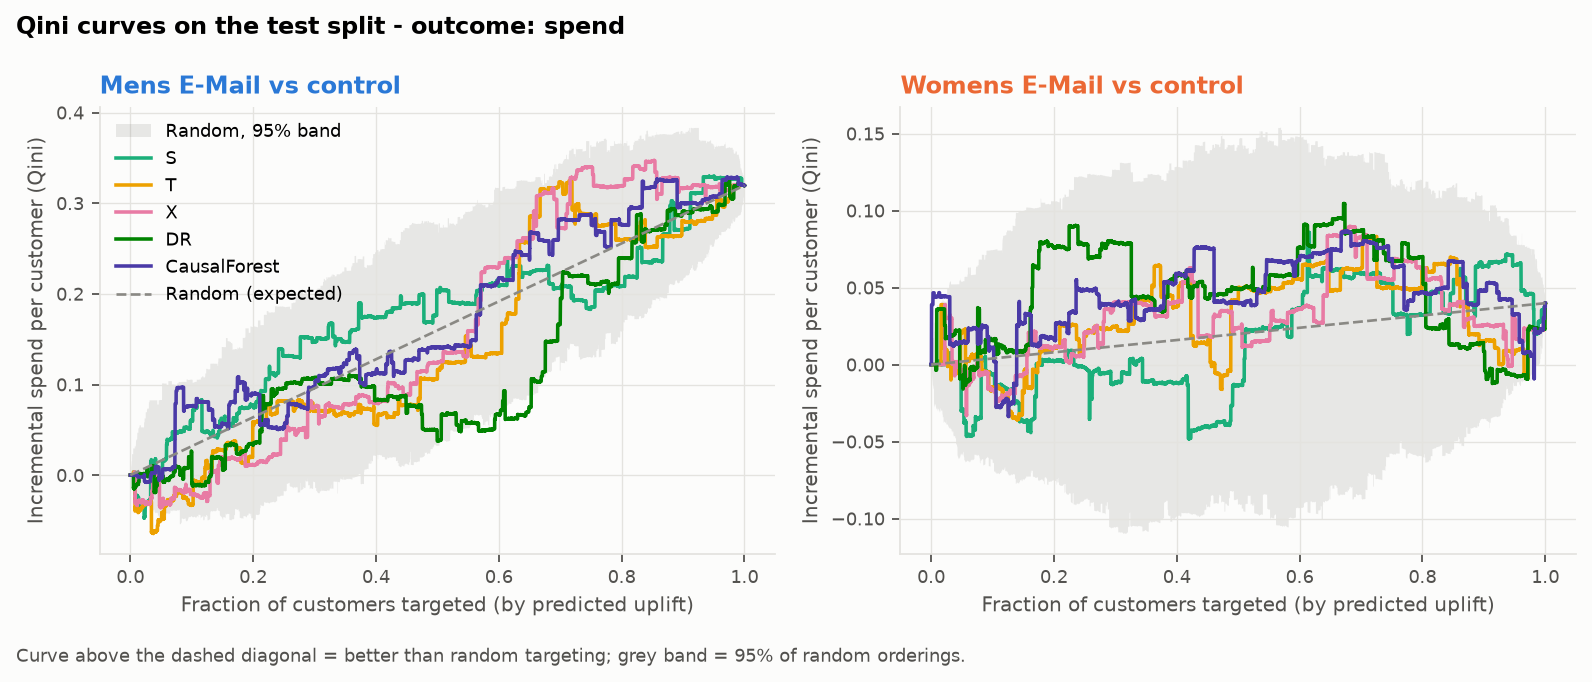
\includegraphics[width=\columnwidth]{figures/qini_curves.png}
\caption{Qini curves for spend on the test split. Every learner stays inside the 95\% band of random
orderings (grey).}
\label{fig:qini}
\end{figure}

\subsubsection{Targeted policies do not beat simple rules}
The targeted policy is indistinguishable from random targeting at every budget and its point
estimate lies \emph{below} ``Mens e-mail to a random subset'' throughout
(Figure~\ref{fig:headline}, left). At $f=1$ it earns $+\$0.31$ \CI{-0.18}{0.83} per customer against
$+\$0.56$ \CI{0.11}{1.03} for the Mens rule; the paired difference is $-\$0.25$ \CI{-0.59}{0.09}. On
visit the targeted policy beats random targeting at 7 of 10 budgets but the Mens rule at only one.

\subsubsection{Solvers}
SCIP proves optimality of \eqref{eq:ip} on all 33 instances up to $n=64{,}000$ (median 45.6\,s). The
Lagrangian heuristic is always feasible, within 0.34\% of the optimum and about $200\times$ faster
(0.23\,s). CP-SAT finds no feasible solution within 30\,s for 9 of 10 budgets at $n=10{,}000$: the
near-integral LP relaxation of the multiple-choice knapsack favours LP-based branch-and-bound.

\begin{figure*}[t]
\centering
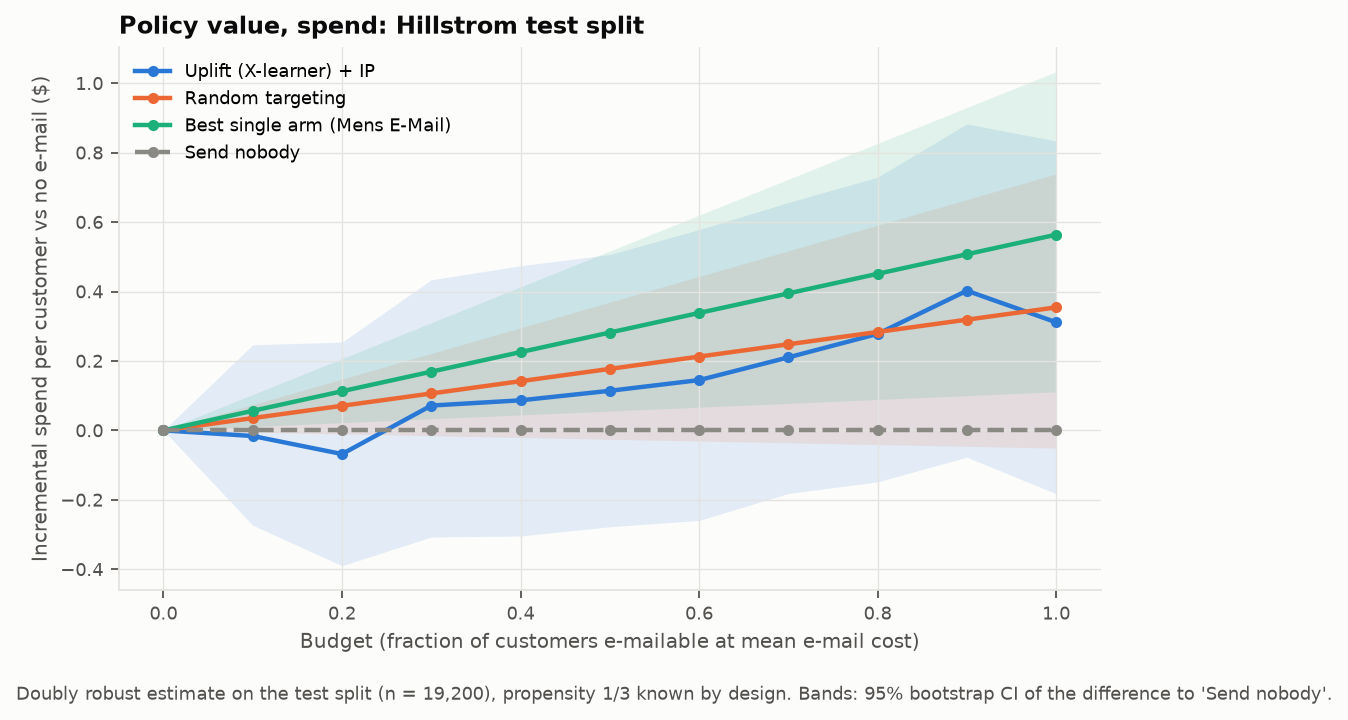
\includegraphics[width=0.49\textwidth]{figures/policy_value_vs_budget.png}\hfill
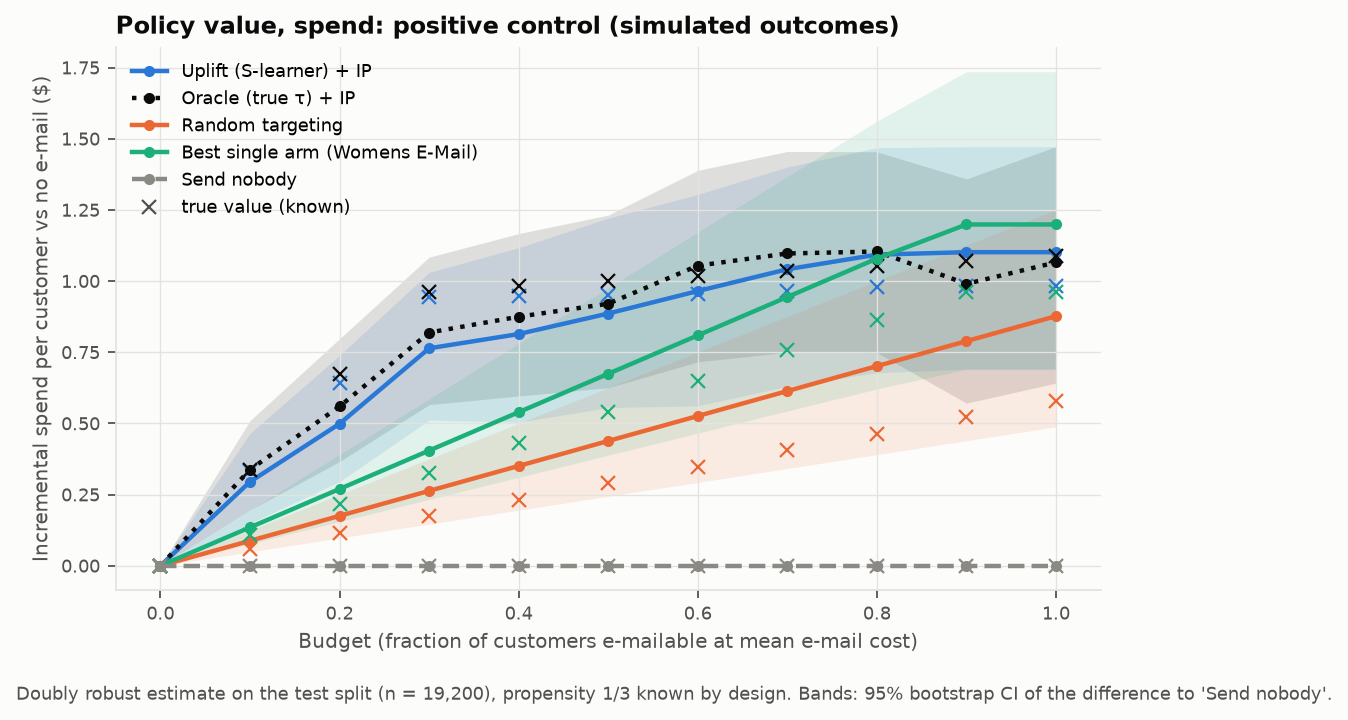
\includegraphics[width=0.49\textwidth]{figures/pc_policy_value_vs_budget.png}
\caption{Incremental spend per customer vs.\ budget (doubly robust, 95\% bootstrap CI). Left: real
Hillstrom outcomes. Right: positive control with the same covariates, assignment and code; $\times$
marks the known true value of each policy.}
\label{fig:headline}
\end{figure*}

\subsection{Positive Control}
The unchanged pipeline finds the planted effect (Table~\ref{tab:pc}, Figure~\ref{fig:headline},
right). For the Womens arm all five learners beat the permutation null ($p\le0.022$) with Qini
values indistinguishable from an oracle that ranks by the true $\tau$, and estimated effects
correlate with the truth at 0.62 to 0.83 (spend) and 0.90 to 0.96 (visit). For the Mens arm the true
effect is constant, so every learner \emph{and} the oracle have Qini near zero. The targeted policy
beats random targeting at 8 of 10 budgets for spend ($+\$0.50$ \CI{0.27}{0.75} at $f=0.3$) and at
all budgets for visit, and its true value is 90 to 98\% of the oracle's. DR intervals cover the true
policy value in 73 of 80 cases; the misses concern nearly identical visit policies and reflect one
test draw about two standard errors high.

\begin{table}[t]
\centering\small
\caption{Positive control, Womens arm: Qini (spend, \$) and correlation of $\tauh$ with the true $\tau$.}
\label{tab:pc}
\begin{tabular}{lrrr}
\toprule
Learner & Qini, spend & $\rho$, spend & $\rho$, visit \\
\midrule
S          & $0.076$ \CI{-.027}{.164} & $0.83$ & $0.96$ \\
T          & $0.095$ \CI{.019}{.166}  & $0.65$ & $0.92$ \\
X          & $0.100$ \CI{.029}{.175}  & $0.75$ & $0.94$ \\
DR         & $0.111$ \CI{.042}{.178}  & $0.62$ & $0.91$ \\
C.\ forest & $0.089$ \CI{.011}{.167}  & $0.65$ & $0.90$ \\
Oracle     & $0.098$ \CI{.013}{.171}  & $1$    & $1$ \\
\bottomrule
\end{tabular}
\end{table}

\subsection{When Does Targeting Pay Off?}
Against the best single arm, which isolates the value of heterogeneity, targeting truly pays from
$h=0.25$ when $n\ge16{,}000$ (e.g.\ $+\$0.06$ \CI{0.05}{0.08} per customer at $n=64{,}000$) and at
every $n$ from $h=0.5$, while at $h=0$ it earns nothing ($-\$0.007$ \CI{-0.013}{0.000};
Figure~\ref{fig:sweep}). Detection lags far behind: at Hillstrom's size a single experiment's DR
interval excludes zero in only 5\%, 25\%, 85\% and 95\% of replications for $h=0.25,0.5,0.75,1$.
Between ``targeting would earn more'' and ``one can show that it does'' lies a band in which the
policy is worth \$0.04 to \$0.23 per customer yet looks like noise. The Hillstrom null is therefore
weak evidence \emph{against} heterogeneity, all the more because Hillstrom's real Womens effect
(\$0.42) is less than half the simulated average (\$0.96).

\begin{figure*}[t]
\centering
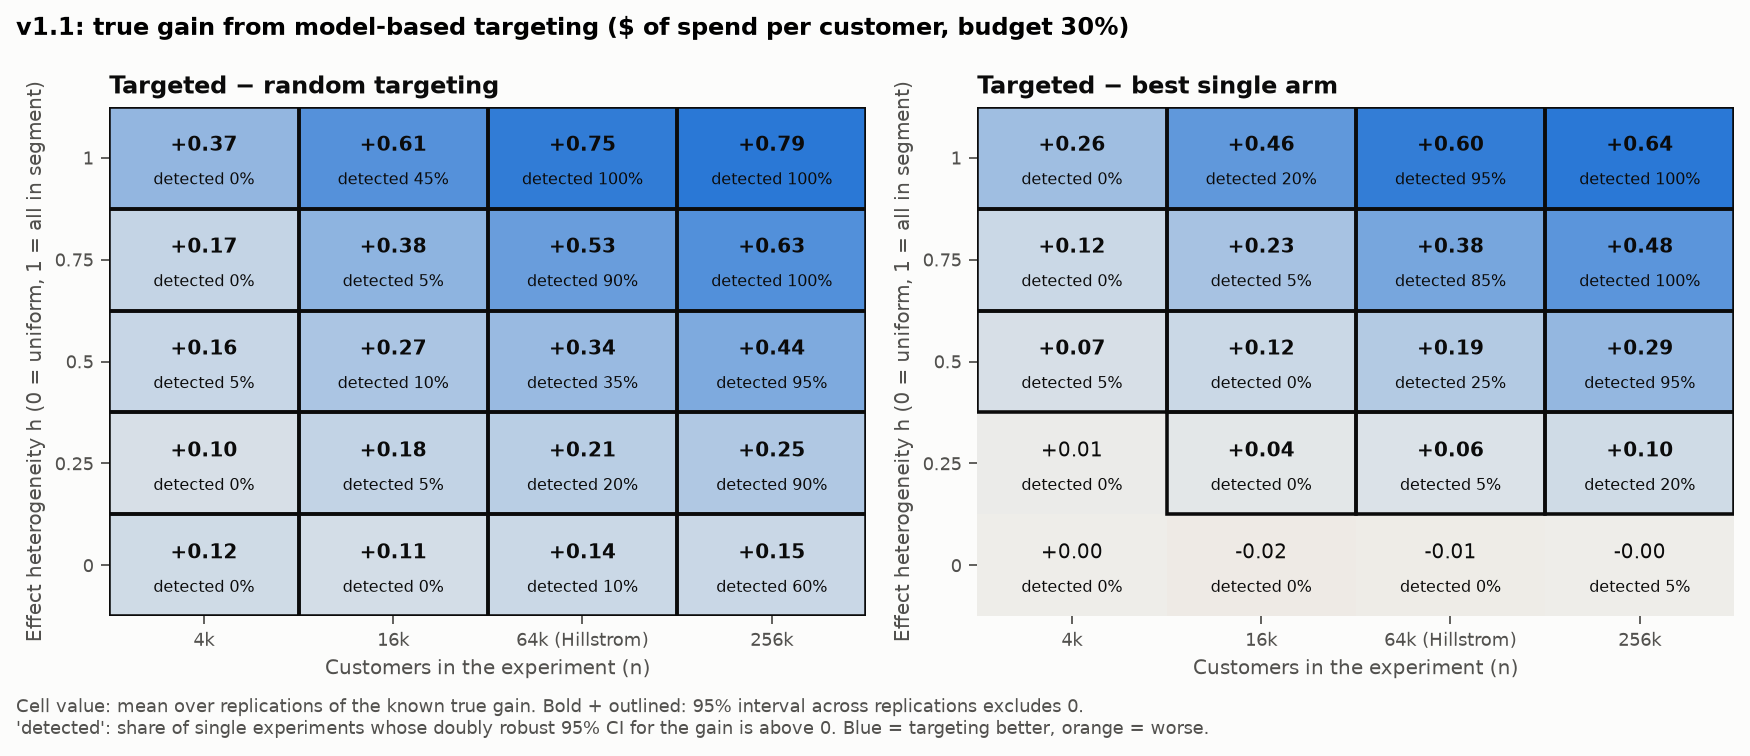
\includegraphics[width=0.92\textwidth]{figures/sweep_heatmap.png}
\caption{True gain from targeting over heterogeneity $h$ and sample size $n$ (mean of 20
replications). Outlined cells: 95\% interval excludes zero. ``Detected'': share of single
experiments whose DR interval lies above zero.}
\label{fig:sweep}
\end{figure*}

\subsection{Profit and Cross-Fitting}
With a profit objective (Figure~\ref{fig:profit}) the targeted policy chooses its own budget: on the
positive control its profit-optimal budget is $f=0.4$ \CI{0.4}{0.65}, matching the true optimum, and
when unconstrained it stops at \$0.047 of spend per customer while earning \$0.211 \CI{0.132}{0.290}
(true \$0.240), more than revenue targeting (\$0.173, true \$0.217). On real Hillstrom no policy
separates from any other (0 of 33 paired comparisons) and the best point estimate is the simplest
rule, Mens e-mail to everyone (\$0.130 \CI{0.045}{0.215}). Repeated cross-fitting \eqref{eq:dml}
narrows intervals by 37 to 58\% relative to the test split while including refit variance, covers
the true profit in 142 of 143 positive-control cases, and establishes that e-mailing pays on real
data ($+\$0.65$ \CI{0.37}{0.93} revenue per customer at $f=1$), but not that \emph{targeting} pays.

\begin{figure*}[t]
\centering
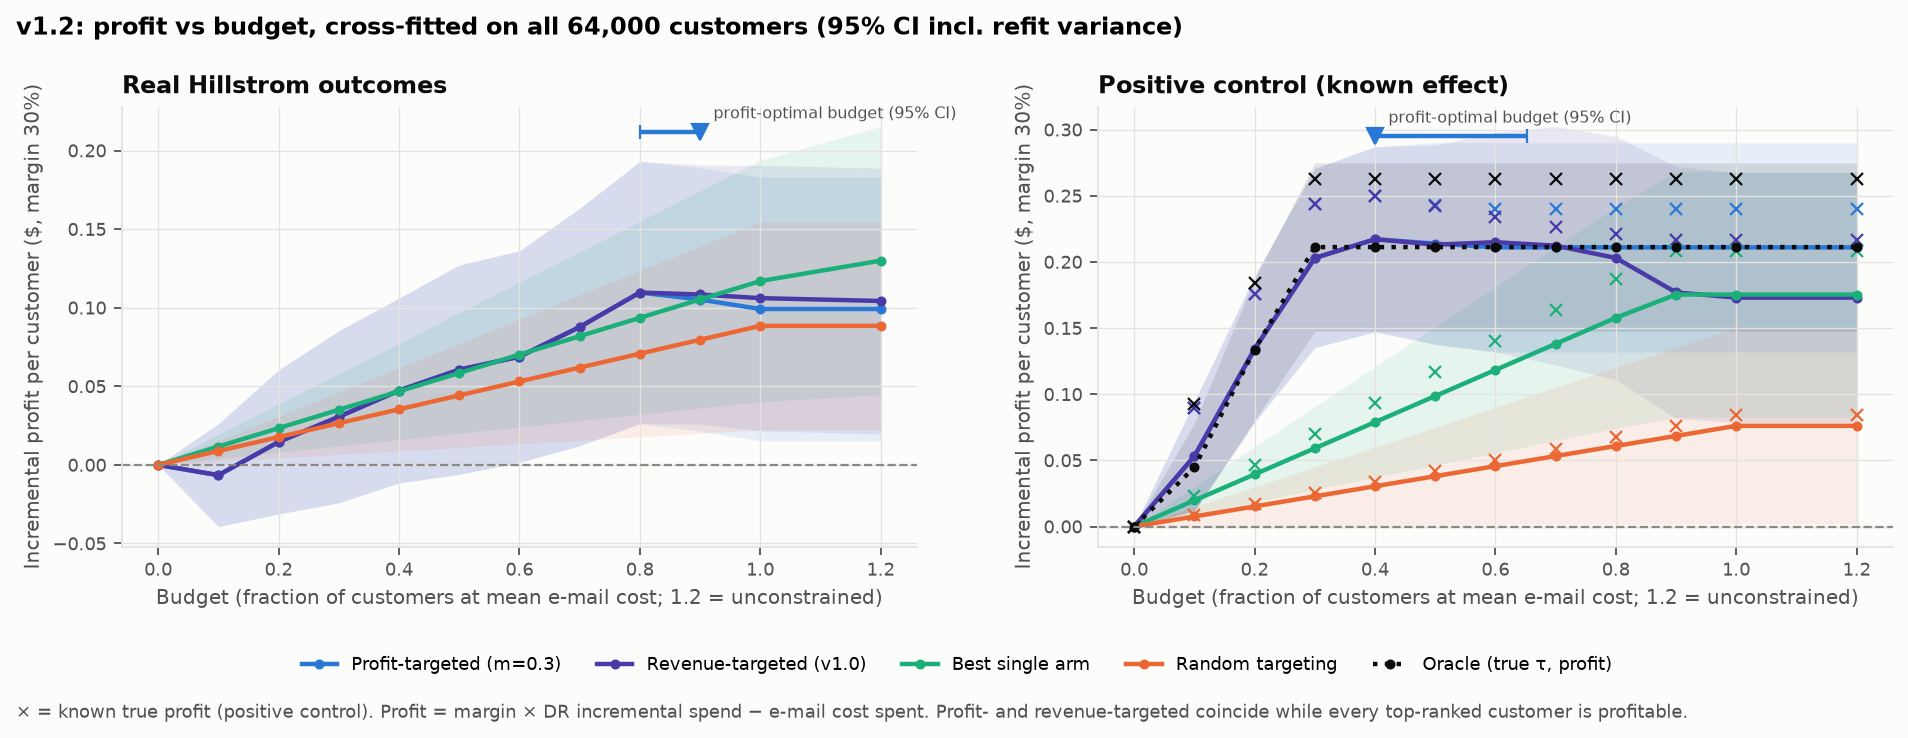
\includegraphics[width=0.92\textwidth]{figures/profit_vs_budget.png}
\caption{Incremental profit vs.\ budget at a 30\% margin, cross-fitted on all customers
($5$ folds $\times$ $10$ repeats). Triangle: profit-optimal budget with 95\% bootstrap interval.}
\label{fig:profit}
\end{figure*}

\subsection{Policy Learning}
Doubly robust policy trees never beat estimate-then-optimise (Figure~\ref{fig:pl}). On real data all
paired differences contain zero, and the depth-2 tree fitted to all customers reads ``Mens e-mail to
everyone except low-spend, very recent customers''. On the positive control, trees lose clearly at a
tight budget ($-\$0.12$ \CI{-0.18}{-0.07} at $f=0.2$): the profitable segment holds 32\% of customers
and a tree can only e-mail whole leaves.

\begin{figure}[t]
\centering
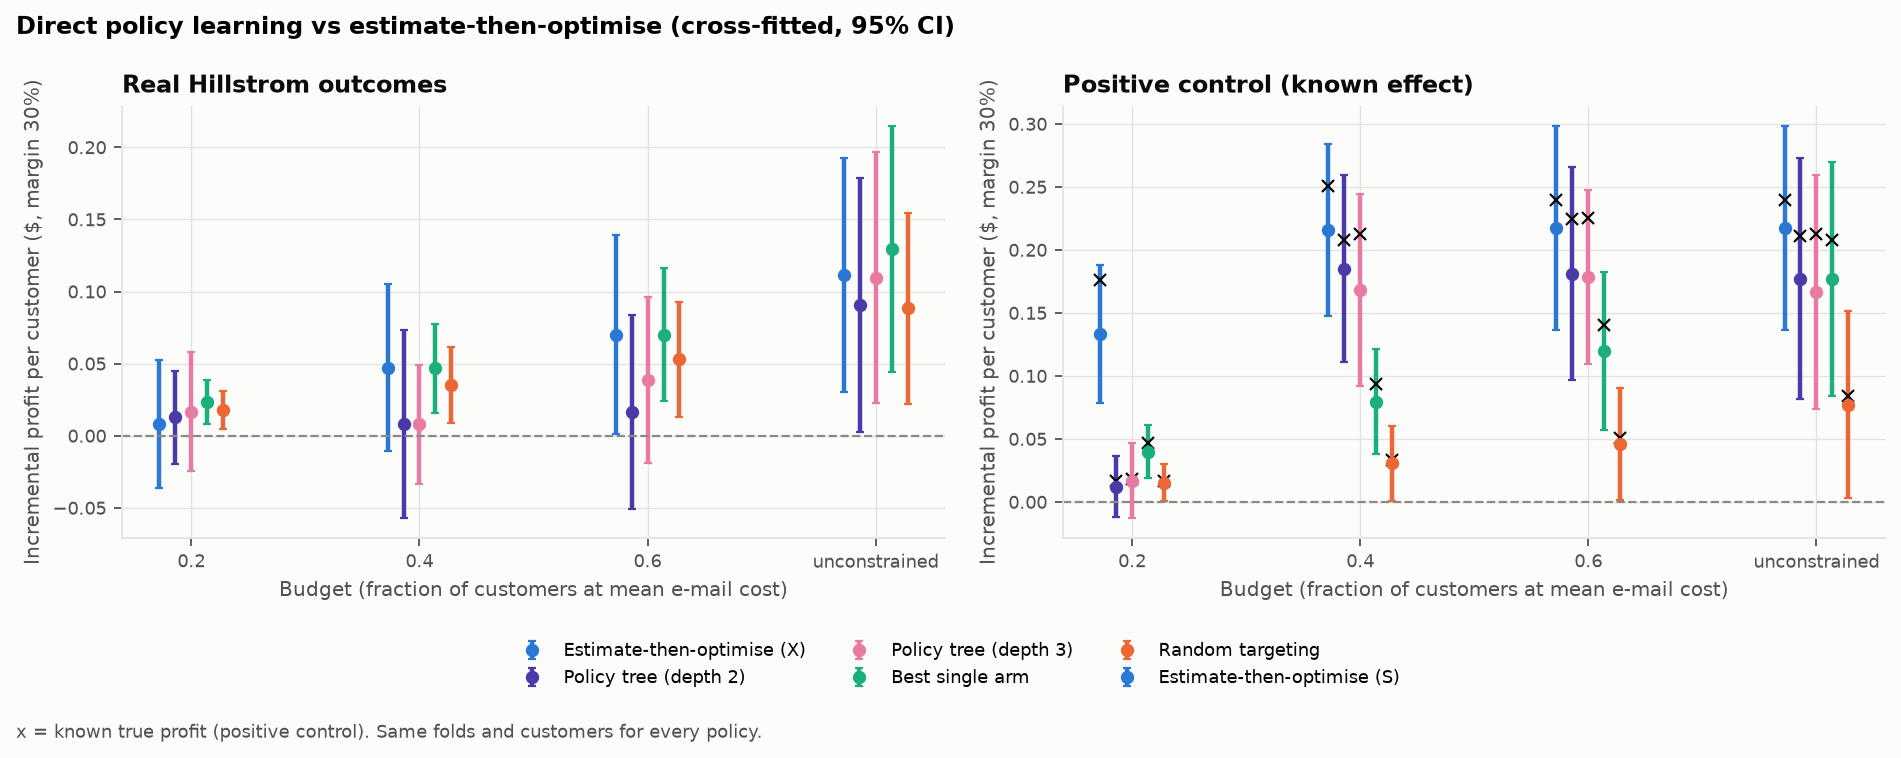
\includegraphics[width=\columnwidth]{figures/policy_learning.png}
\caption{Policy trees vs.\ estimate-then-optimise on identical cross-fitting folds ($5\times5$).}
\label{fig:pl}
\end{figure}

\subsection{Chance Constraints}
\subsubsection{The optimiser's curse}
Under random voucher uptake, the mean-budget policy overruns its budget in 63 to 85\% of campaigns
and the plug-in chance-constrained policy in 14 to 32\% (Figure~\ref{fig:chance}), at an 8 to 18\%
loss of profit, missing the 5\% target it believes it meets. Estimated uptake is calibrated overall
(0.012 vs.\ 0.012) but about 10\% too low among the customers the allocator selects (0.026 vs.\ 0.028
to 0.029): customers who look cheap are partly cheap by estimation error \citep{smith2006}.

\begin{figure}[t]
\centering
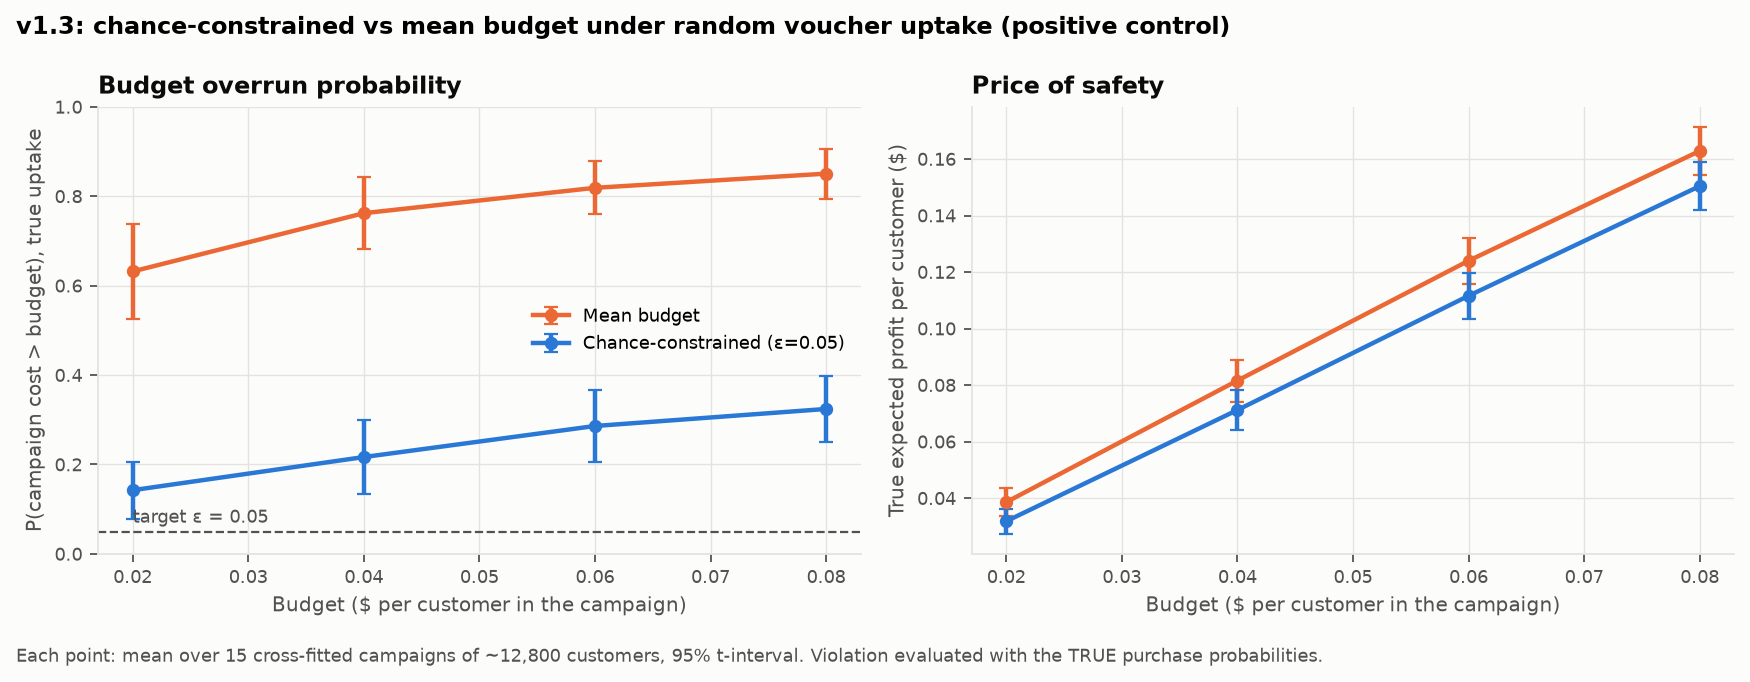
\includegraphics[width=\columnwidth]{figures/chance_constraint.png}
\caption{Overrun probability (true uptake) and true profit, positive control, 15 campaigns.}
\label{fig:chance}
\end{figure}

\subsubsection{Repairing the curse}
Recalibration barely helps (Table~\ref{tab:chance15}, Figure~\ref{fig:chance15}): $\hat\kappa$ comes
out at about 1 while the true ratio among selected customers is 1.08 to 1.12, because a 10\% bias is
below what IPW on a few hundred matched purchases can resolve. The bootstrap bound holds the target
with room to spare (overrun at most 0.8\%) but gives up 16 to 19\% of profit.

\begin{table}[t]
\centering\small
\caption{True overrun probability on the positive control (95\% CI, 15 campaigns) and true profit
per customer for the plug-in constraint vs.\ the bootstrap bound.}
\label{tab:chance15}
\setlength{\tabcolsep}{3pt}
\begin{tabular}{lrrrr}
\toprule
Budget & Plug-in & Recalibrated & Bootstrap & Profit \\
\midrule
0.02 & $0.14$ \CI{.08}{.20} & $0.11$ \CI{.05}{.17} & $0.008$ & $0.032\to0.026$ \\
0.04 & $0.22$ \CI{.14}{.30} & $0.19$ \CI{.11}{.27} & $0.003$ & $0.071\to0.058$ \\
0.06 & $0.29$ \CI{.21}{.36} & $0.21$ \CI{.12}{.30} & $0.001$ & $0.112\to0.092$ \\
0.08 & $0.32$ \CI{.25}{.40} & $0.24$ \CI{.15}{.34} & $0.000$ & $0.150\to0.126$ \\
\bottomrule
\end{tabular}
\end{table}

\begin{figure}[t]
\centering
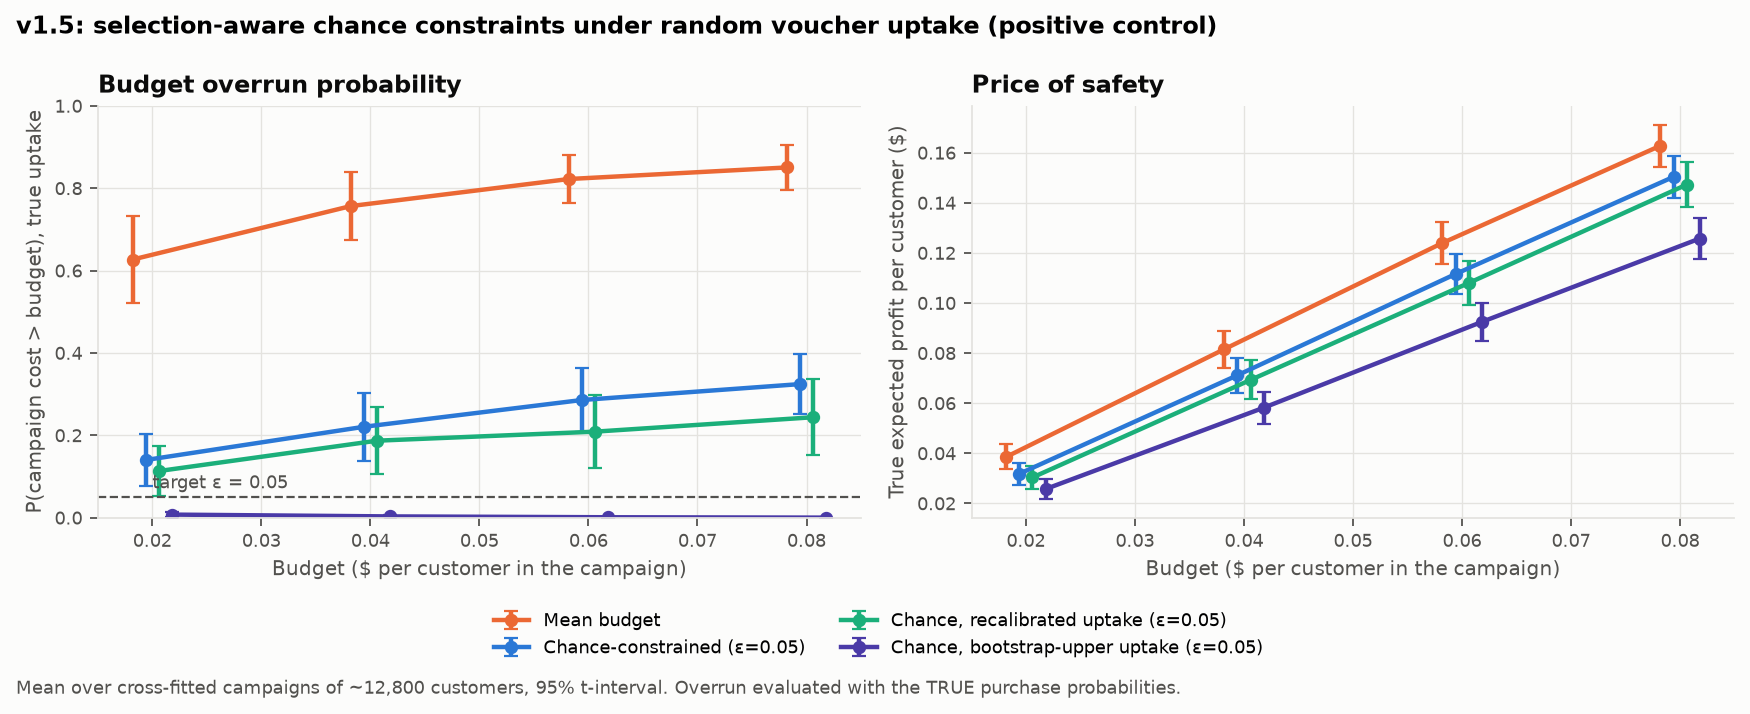
\includegraphics[width=\columnwidth]{figures/chance15.png}
\caption{Overrun probability and true profit for the plug-in, recalibrated and bootstrap-bound
chance constraints (positive control).}
\label{fig:chance15}
\end{figure}

\subsection{Sequential Allocation}
The bandit earns 68\% of the oracle's profit when effects are heterogeneous, against 47 to 60\% for
experiment-then-target (Table~\ref{tab:seq}, Figure~\ref{fig:seq}). It beats $k=1$ by \$0.027
\CI{0.001}{0.054} and $k=4$ by \$0.054 \CI{0.046}{0.062} per customer; against $k=2$ the gain,
\$0.021 \CI{-0.002}{0.043}, is not significant. Its main advantage is robustness: an interval four
times narrower than $k=1$'s. With homogeneous effects the bandit is indistinguishable from
$k\in\{1,2\}$, so adaptivity costs nothing when there is nothing to learn.

\begin{table}[t]
\centering\small
\caption{Total true profit per customer over a 64{,}000-customer campaign (95\% CI, 20 replications).}
\label{tab:seq}
\setlength{\tabcolsep}{4pt}
\begin{tabular}{lrr}
\toprule
Policy & Heterogeneous & Homogeneous \\
\midrule
Oracle (true $\tau$)         & $0.263$ & $0.070$ \\
Thompson bandit              & $\mathbf{0.178}$ \CI{.172}{.184} & $0.054$ \CI{.050}{.058} \\
Exp.-then-target, $k=1$      & $0.150$ \CI{.123}{.177} & $0.052$ \CI{.041}{.064} \\
Exp.-then-target, $k=2$      & $0.157$ \CI{.135}{.179} & $0.050$ \CI{.044}{.056} \\
Exp.-then-target, $k=4$      & $0.124$ \CI{.117}{.131} & $0.045$ \CI{.045}{.045} \\
Random targeting             & $0.025$ & $0.025$ \\
\bottomrule
\end{tabular}
\end{table}

\begin{figure*}[t]
\centering
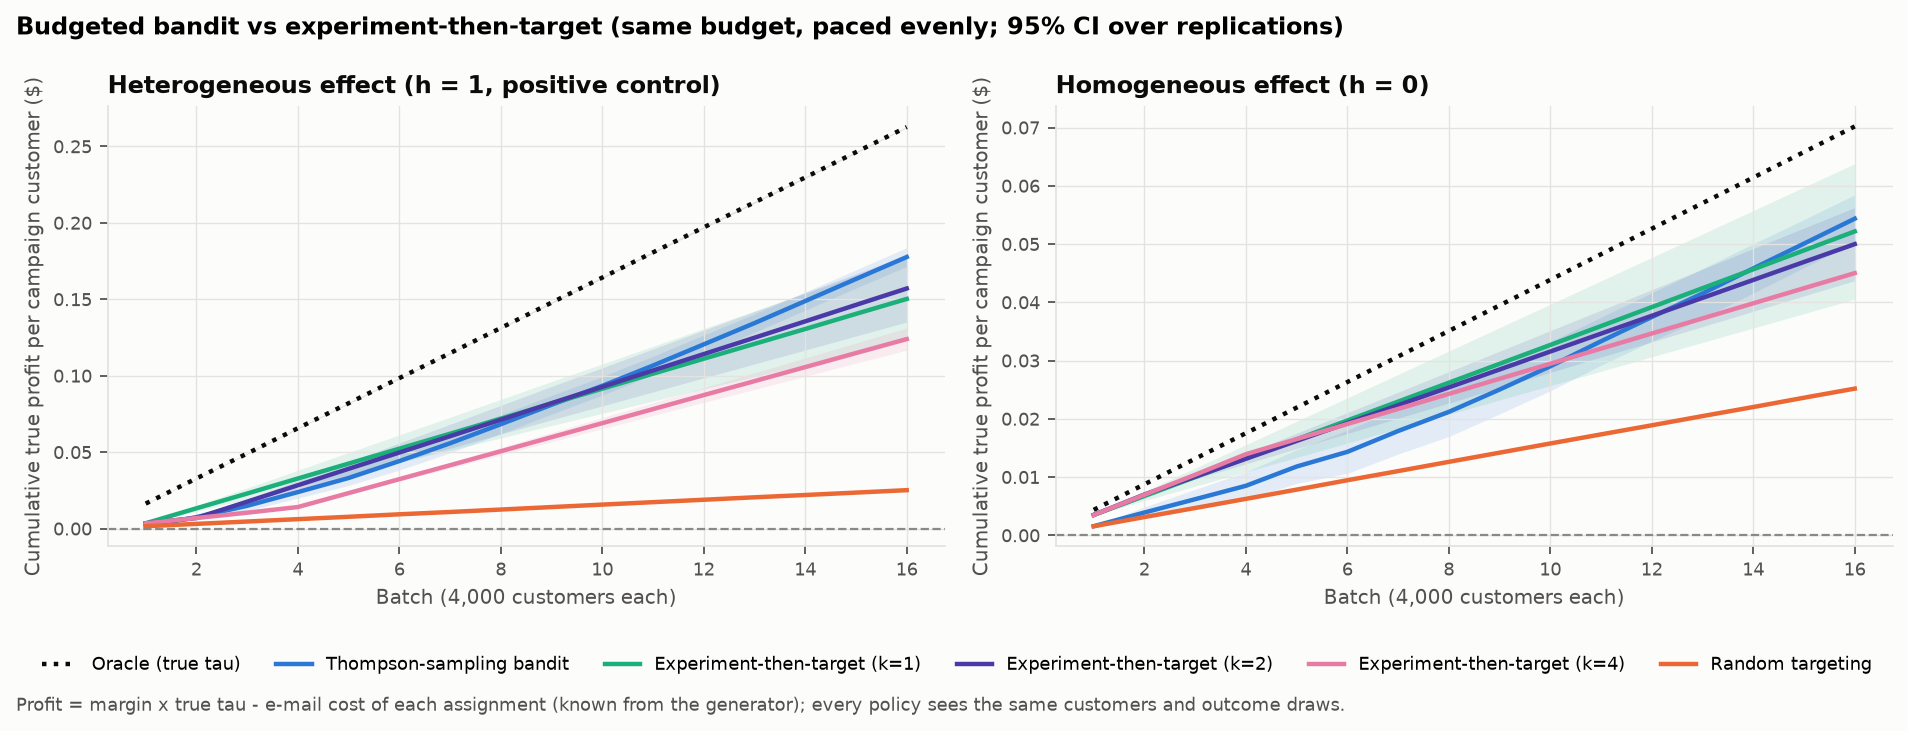
\includegraphics[width=0.92\textwidth]{figures/sequential.png}
\caption{Cumulative true profit per campaign customer over 16 batches (95\% CI over replications).}
\label{fig:seq}
\end{figure*}

\subsection{Robustness Checks}
A deliberately confounded sample biases the naive visit effect by $+1.8$\,pp; IPW with an estimated
propensity and AIPW recover the RCT value within 0.2\,pp. Allocating on a lower confidence bound of
$\tauh$ lowers both mean and 5th-percentile policy value at every budget. Sentence-embedding
features \citep{reimers2019} change Qini by $+0.019$ \CI{-0.042}{0.081} and $-0.022$
\CI{-0.052}{0.010}: the text restates the tabular covariates.

% =========================================================================================
\section{Conclusions}
\label{sec:conclusions}

\subsection{Summary of Contributions}
This project delivers an end-to-end, multi-arm, budget-constrained uplift pipeline with doubly
robust evaluation, run under a pre-registration-by-commit protocol. Its central finding on Hillstrom
is negative for spend; a positive control shows that this is a property of the data rather than of
the method; and a heterogeneity sweep quantifies how weak that negative evidence is. Five further
studies show that a profit objective chooses its own budget, that repeated cross-fitting sharpens
policy evaluation, that policy trees do not beat estimate-then-optimise, that plug-in chance
constraints fail through the optimiser's curse while a conservative bound holds, and that a
budgeted bandit beats or ties one-shot experimentation.

\subsection{Discussion}
For practitioners the results suggest four habits: evaluate targeted policies against the best
single arm, not only against random targeting; size experiments for \emph{policy} differences,
which are much harder to detect than average effects; distrust plug-in constraints built on the
same model that selected the customers; and prefer a conservative bound to a data-driven correction
when uptake is rare.

\subsection{Limitations}
SUTVA is assumed throughout (no household spill-over or cannibalisation). Outcomes cover two weeks
after a single 2008 campaign, with no long-run effects, fatigue or unsubscribes. Costs, margin and
voucher value are assumptions. The positive control is only as realistic as its generator: additive
effects, a simple segment rule on observed covariates, and amounts independent of $X$. Learners and
LightGBM parameters were fixed from the first release onwards. Several comparisons across budgets and
outcomes are reported without multiplicity correction.

\subsection{Future Work}
A scale check on the Criteo uplift data \citep{diemert2018} was planned but not run because all known
download locations were unavailable. Other natural extensions are adaptive budget pacing for the
bandit, uptake models calibrated on a dedicated holdout, a profit objective with returns and
long-run effects, and multiplicity-adjusted comparisons across budgets.

% =========================================================================================
\section{Broader Impact Statement}
\label{sec:impact}

Targeting decides who receives an offer, so it can also decide who does not: a profit-optimal policy
may systematically exclude groups that look less responsive, and covariates can act as proxies for
protected characteristics. This project uses only purchase-history covariates from a public,
anonymised dataset, but any deployment should audit who is excluded and why. The main finding cuts
the other way as well: on these data, simple rules perform as well as targeted ones, so the extra
data collection and modelling that targeting requires would not be justified. More generally, the
pre-registration protocol and the public decision log are offered as a way to make analytics claims
checkable rather than persuasive.

\bibliographystyle{apacite}
\bibliography{references}

\end{document}
